\documentclass{journal}[IEEEtran, twocolumn]             % No modificar

% PASO 1. Reemplace "Práctica 1" por el número de la práctica que corresponda
\newcommand{\dochead}{Práctica 2}     

% PASO 2. Reemplace "TÍTULO PRÁCTICA" por el título de la práctica que corresponda.
\newcommand{\docsubhead}{PSD de señales aleatorias}  

% PASO 3. Reemplace "B1A - 02" por el grupo de la asignatura y el número de su grupo de laboratorio
\newcommand{\teamname}{C1}     

% PASO 4. OPCIONAL: Reemplace "\docsubhead \docsubhead" por el título del documento en caso de requerirse.
\newcommand{\titulo}{\dochead: \docsubhead}      

% PASO 5. Reemplace "31 de diciembre de 2030" por la fecha de su documento
\newcommand{\fecha}{12 de octubre de 2024}      

% To load packages
\usepackage[T1]{fontenc}
\usepackage[utf8]{inputenc} 
\usepackage[spanish]{babel}
\usepackage[letter,left=2.0cm,top=2.0cm,right=2.0cm,bottom=4.0cm]{geometry}
\usepackage{amsmath}
\usepackage{amsfonts}
\usepackage{fancyhdr}
\usepackage{fancyvrb}
\usepackage{listings}
\usepackage{array}
\usepackage{graphicx,color,enumerate}	
\usepackage{multirow} 
\usepackage{multicol}
\usepackage{authblk}
\usepackage{charter}    % Font typeface
\usepackage{titling}
\usepackage{url}
\usepackage{hyperref}
\usepackage{xcolor}
\usepackage{booktabs}

\definecolor{uisgreen}{RGB}{125,194,3}
\definecolor{gray97}{gray}{.97}
\definecolor{gray75}{gray}{.75}
\definecolor{gray45}{gray}{.45}

\setlength{\droptitle}{-1.8cm}
\pagestyle{fancy}

%%% Header definition
\headheight=60pt 						% header height 
\renewcommand{\headrulewidth}{4pt}
\let\oldheadrule\headrule% Copy \headrule into \oldheadrule
\renewcommand{\headrule}{\color{uisgreen}\oldheadrule}

\fancyhead[L]							% left header 
{	\begin{minipage}{2.5cm}
		
\includegraphics[scale=0.3]{./figs/uislogohoriz.png} 
	\end{minipage}	
	\begin{minipage}{5cm}
	    \color{uisgreen}
	    \footnotesize {\textsf{Universidad Industrial de Santander\\ 
				Escuela de Ingenierías Eléctrica, \\
				Electrónica y de Telecomunicaciones	}}	
	\end{minipage}
}
\fancyhead[R] { 							%la "C" indica al centro
	\begin{minipage}{8cm}
	    \color{uisgreen}
	    \begin{flushright}
    	    \small{\textsf{Laboratorio de COMUNICACIONES I (27139)}} \\
            \normalsize{\textsf{\dochead: \textbf{\docsubhead}}} \\
    	    \small{\textsf{Grupo: \textbf{\teamname}}}
	    \end{flushright}
    \end{minipage}
    \begin{minipage}{1.2cm}
		
\includegraphics[width=1.0\textwidth]{./figs/logoE3T.png} 
	\end{minipage}	
}
%%% End header definition

\lstset{ frame=Ltb,
     framerule=0pt,
     aboveskip=0.5cm,
     framextopmargin=3pt,
     framexbottommargin=3pt,
     framexleftmargin=0.4cm,
     framesep=0pt,
     rulesep=.4pt,
     backgroundcolor=\color{gray97},
     rulesepcolor=\color{black},
     %
     stringstyle=\ttfamily\color{red!50!brown},
     showstringspaces = false,
     basicstyle=\small\ttfamily,
     commentstyle=\color{gray45},
     keywordstyle=\color{blue}\bfseries,
     %
     numbers=left,
     numbersep=15pt,
     numberstyle=\tiny,
     numberfirstline = false,
     breaklines=true,
   }

% minimizar fragmentado de listados
\lstnewenvironment{listing}[1][]
   {\lstset{#1}\pagebreak[0]}{\pagebreak[0]}

\lstdefinestyle{consola}
   {basicstyle=\scriptsize\bf\ttfamily,
    backgroundcolor=\color{gray75},
   }

\lstdefinestyle{C}
   {language=C,}             % No modificar


\begin{document}                    % No modificar

\title{\textbf{\titulo}}            % No modificar

% PASO 6. Agregar aquí el nombre y código de los autores.  
\author{
Carlos Alberto Cetina - 2215583\\
Brayan Julian Niño Hurtado - 2172301\\
Sergio Camilo Santos - 2172315\\
\href{https://github.com/scsantosdth/CommunicationsII_2024_2_scb.git}{https://github.com/scsantosdth/CommunicationsII_2024_2_scb.git}
}

\affil{\small{Escuela de Ingenierías Eléctrica, Electrónica y de Telecomunicaciones} \\ % No modificar
\small{Universidad Industrial de Santander}} % No modificar

\date{\fecha}                       % No modificar

\maketitle                          % No modificar
\thispagestyle{fancy}          % No modificar

%---------------------------------------------------------------
% PASO 7. **..**...****INICIE SU DOCUMENTO DESDE AQUI***...**...
%%%%% A PARTIR DE AQUÍ EDITE EL DOCUMENTO PARA AGREGAR TODO EL CONTENIDO REQUERIDO PARA EL ENTREGABLE CORRESPONDIENTE
%%%%  Todo el contenido a partir de este punto es SOLAMENTE ILUSTRATIVO.
%
% Para sus imformes, BORRE TODO el contenido de aquí en adelante  EXCEPTO la última línea que contiene el comando: \end{document}


\color{black}

\begin{multicols}{2}

\begin{abstract}
    This report presents the analysis and calculation of the Power Spectral Density (PSD) of random signals using GNURadio as the main tool. Both native GNURadio blocks and custom functions were employed to generate signals and calculate their PSD. The main objective is to understand the spectral structure of the signals and their energy distribution as a function of frequency, while internalizing key concepts related to random signals and averaging techniques.
\end{abstract}

\section{Introducción}
   En este laboratorio, se estudiará el uso de herramientas y funciones de GNURadio para calcular la PSD de señales aleatorias. Implementando no solo bloques ya disponibles en la plataforma, sino que también funciones personalizadas para generar y analizar señales, comprendiendo mejor los conceptos de señales aleatorias y el análisis espectral.


\section{Metodología}
\subsection{Parte A: Comprobar el funcionamiento del frujograma}
Se implementó el flujograma propuesto analizando el comportamiento de una señal binaria aleatoria bipolar de forma rectangular. Se obsrvó su formama en el tiempo, además de calcular su Densidad Espectral de Potencia (PSD). Se obtuvo la frecuencia de muestreo, ancho de banda y rata de bits, para diferentes valores de Sps (Samples per symbol) ajustando el valor de la variable h la cual define el tamaño del vector.



\subsection{Parte B: Comprobar como es el ruido blanco}
Para comprobar el ruido blanco en tiempo y en PSD, se configuraron dos bloques 'Virtual Source'  denominados p4 y p5. Se generó ruido blanco utilizando un bloque 'Noise Source'  y se realizaron varias priuebas ajustando la amplitud. 

 
\subsection{Parte C: Análisis de señal de una imagen}
En esta parte, se evaluó el comportamiento de la señal cuando los bits provienen de una fuente del mundo real. Para ello, se modificó el flujograma reemplazando el bloque "Random Source" por los bloques "File Source" y "Unpack K Bits", permitiendo la lectura del archivo "rana.jpg" y la extracción de sus bits. Posteriormente, se realizaron varias pruebas para observar la representación de la señal en el dominio temporal y su Densidad Espectral de Potencia (PSD). Este análisis permitió visualizar cómo se comporta la señal en comparación con una fuente aleatoria, basándose en las gráficas obtenidas.

\subsection{Parte D: Análisis de señal de un micrófono}
Se estudió el comportamiento de la señal en los dominios temporal y frecuencial utilizando datos de audio provenientes de un micrófono. Para ello, se configuró el bloque "File Source" para leer el archivo "sonido.wav", lo que permitió capturar los bits que representan la grabación. A través de gráficas generadas, se registraron observaciones y conclusiones que resaltan las diferencias en la estructura de la señal y su comportamiento espectral, en especial la Densidad Espectral de Potencia (PSD), en comparación con fuentes de datos más aleatorias.

\subsection{Parte E: Preguntas de control}
Preguntas de auto control sobre el flujograma randombinayrectsignal.grc
    
\section{Resultados}
\subsection{Parte A: Comprobar el funcionamiento del frujograma}

Como resultado, se logró visualizar la representación temporal y la Densidad Espectral de Potencia (PSD) de una señal binaria bipolar aleatoria (\textbf{Figura \ref{fig:1}}). Lo que permitió examinar su comportamiento, validando los parametros con las siguientes relaciones.

    \begin{center}
    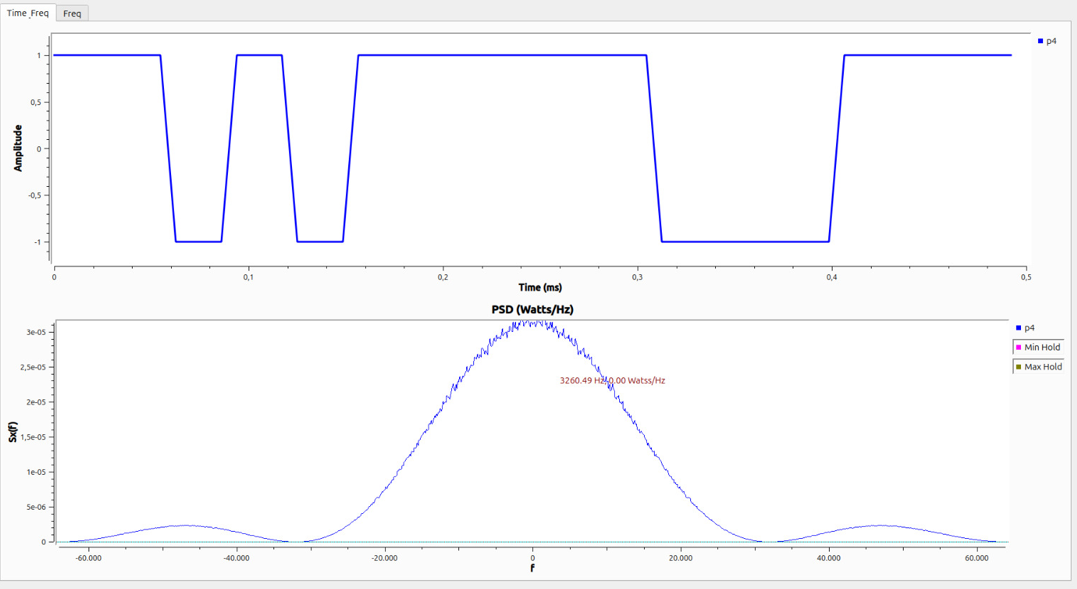
\includegraphics[width=0.45\textwidth]{figs/F1.png}
    \caption{Figura 1: Resultao gráfica en tiempo y frec (Sps=4)}
    \label{fig:1}
    \end{center}
    
El ancho de banda de una señal binaria aleatoria bipolar se puede calcular usando la fórmula \( BW = R_b \times Sps \), donde \( R_b \) es la tasa de bits y \( Sps \) es el número de muestras por símbolo. A medida que se aumenta el valor de \( Sps \), la frecuencia de muestreo también aumenta, lo que a su vez amplía el ancho de banda necesario para transmitir la señal sin distorsiones. Este cálculo es clave para determinar el rango de frecuencias en el que la señal puede ser transmitida eficazmente sin interferencias. \cite{comu}.

    \begin{center}
    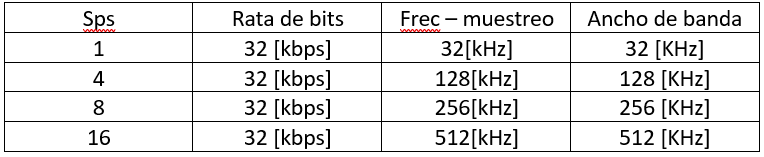
\includegraphics[width=0.45\textwidth]{figs/F2.png}
    \caption{Tabla 1: Resultado flujograma}
    \label{tab:1}
    \end{center}
    
Con los resultados obtenidos (\textbf{Tabla \ref{tab:1}}), se observó que al incrementar el número de muestras por símbolo (Sps), también aumenta la frecuencia de muestreo ($f_s$). Este aumento se debe porque al incrementar el Sps, se mejora la resolución temporal de la señal, dividiendo cada símbolo en más muestras. Esto requiere una mayor frecuencia de muestreo para capturar con precisión los detalles de cada símbolo y representar la señal adecuadamente sin pérdida de información. 

Sin embargo, el bit rate (Rb) se mantiene constante porque, aunque aumente el número de muestras que describen un símbolo, esto no cambia la cantidad de símbolos que se envían en un segundo. ya que la frecuencia muestreo ($f_s$) crece para representar más muestras por símbolo en el mismo tiempo.


\subsection{Parte B: Comprobar como es el ruido blanco}

    \begin{center}
    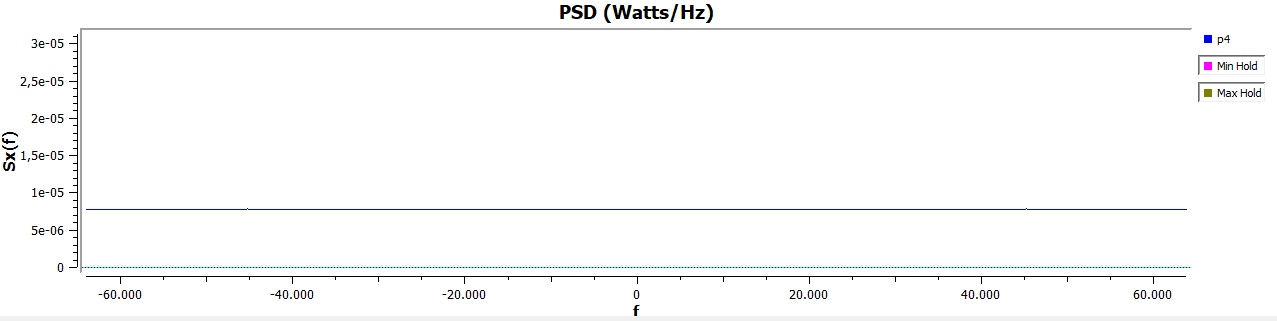
\includegraphics[width=0.45\textwidth]{figs/F3.png}
    \caption{Figura 2: PSD del ruido blanco}
    \label{fig:2}
    \end{center}

En los resultados obtenidos en la (\textbf{Figura \ref{fig:2}}), se observó que al aumentar la amplitud del bloque "Noise Source", la Densidad Espectral de Potencia ($S_x(f)$) también crece de manera proporcional. Este comportamiento ocurre porque al incrementar la amplitud de la señal, aumenta la energía total contenida en ella, lo que se traduce en un incremento de la potencia. El aumento de potencia genera un incremento de la ganancia, directamente relacionado con la temperatura equivalente del ruido en el receptor. Dado que la Densidad Espectral de Potencia está definida por $N_0/2$, donde $N_0 = k \cdot T_e$ (siendo $T_e$ la temperatura equivalente y $k$ la constante de Boltzmann), al aumentar la temperatura, el valor de $N_0$ se incrementa. Esto explica por qué a mayor amplitud, mayor es la temperatura, la potencia y, por lo tanto, el valor de $S_x(f)$. Además, la gráfica de $S_x(f)$ constante a lo largo de todas las frecuencias confirma la naturaleza del ruido blanco, caracterizado por un espectro de potencia uniforme y un ancho de banda teóricamente infinito. \cite{libro1}


\subsection{Parte C: Análisis de señal de imagen}

    \begin{center}
    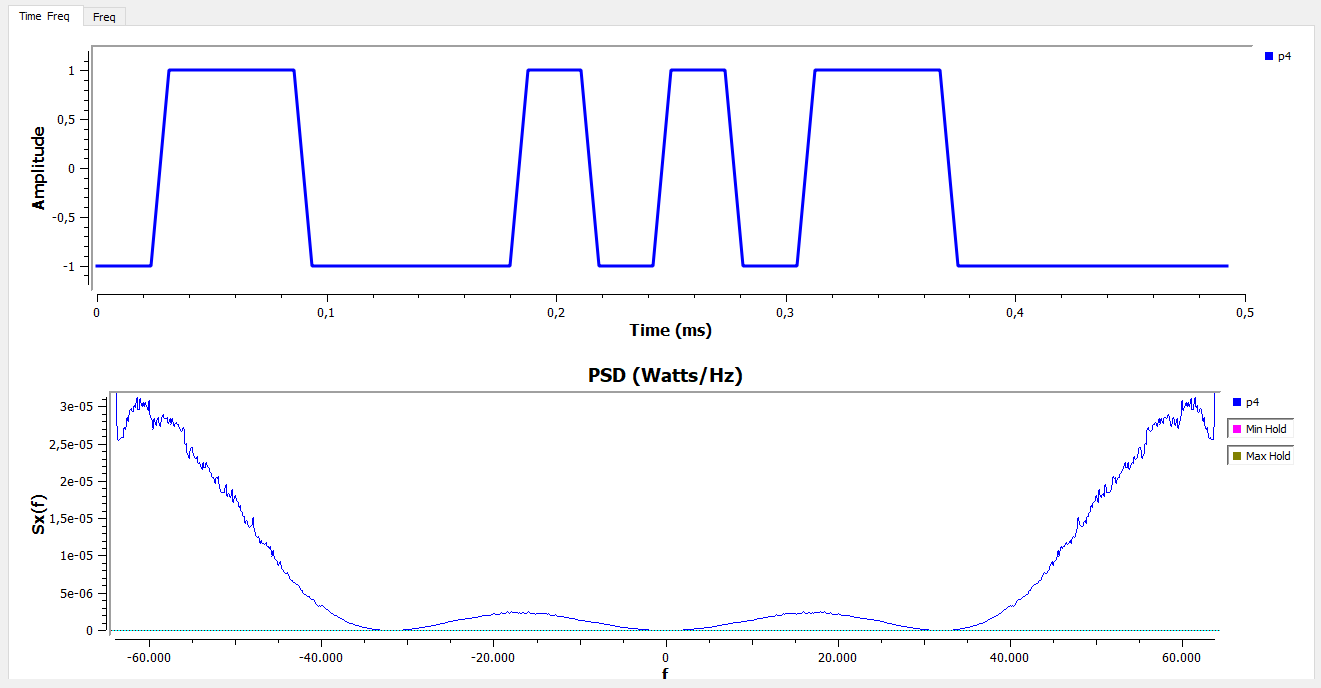
\includegraphics[width=0.45\textwidth]{figs/F4.png}
    \caption{Figura 3: Gráficas de tiempo y PSD señal de imagen}
    \label{fig:3}
    \end{center}


Como resultado, para las señales, cuando la fuente es una imagen, se obtuvieron gráficas similares a las de una señal binaria aleatoria bipolar, lo que se atribuye al proceso de codificación de datos. Al transformar una imagen en datos binarios, se genera una secuencia de bits que puede parecer aleatoria, especialmente en imágenes con variaciones de intensidad. Esto resulta en patrones de 0s y 1s que carecen de una estructura clara en el dominio temporal, similar a las señales binarias aleatorias. Asimismo, la Densidad Espectral de Potencia (PSD) de estas señales es comparable, ya que ambas comparten la naturaleza binaria de los datos. La conversión a bits distribuye la energía en el espectro de manera uniforme, produciendo una PSD que muestra un comportamiento similar, independientemente de la fuente de los datos tal y como se muestra en la (\textbf{Figura \ref{fig:3}}).


\subsection{Parte D: Análisis de señal de un micrófono}


    \begin{center}
    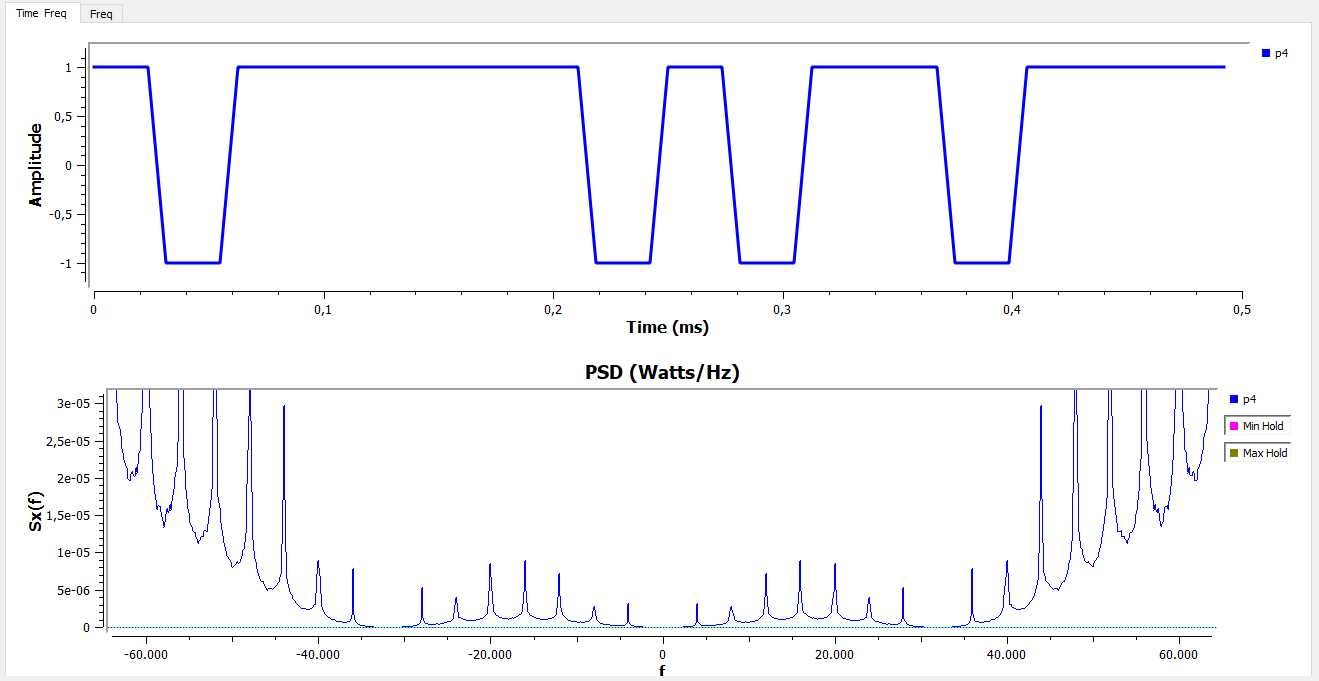
\includegraphics[width=0.45\textwidth]{figs/F5.png}
    \caption{Figura 4: Gráficas de tiempo y PSD señal de sonido}
    \label{fig:4}
    \end{center}
    
Al analizar en la (\textbf{Figura \ref{fig:4}}) la señal proveniente del micrófono, representada en el archivo de audio ``sonido.wav'', se observó que en el dominio temporal la señal no mostró diferencias significativas en comparación con una señal binaria aleatoria bipolar. Esto sugiere que la conversión del audio a bits binarios genera un patrón de 0s y 1s que puede parecer similar a una secuencia aleatoria, ya que en la representación temporal no se destaca la estructura del contenido del sonido. Sin embargo, en el dominio frecuencial, la Densidad Espectral de Potencia (PSD) reveló diferencias notables. Se observó una serie de pulsos o picos a lo largo del espectro, y el número de estos picos correspondía directamente con el número de bits configurados en el bloque 'Unpack k bits'. Esto sucede porque, al aumentar el número de bits en la descomposición de la señal, se incrementa el nivel de detalle en la representación binaria, lo que resulta en una mayor cantidad de transiciones de 0s y 1s, que se reflejan en la PSD como picos adicionales. Estos picos indican un incremento en la cantidad de información codificada por cada transición de bits, lo cual afecta la resolución y estructura espectral.

\subsection{Parte E: Preguntas de control}
\begin{itemize}
    \item[a.] La combinación de bloques mostrada en la figura realiza la siguiente operación: 
    Un bloque ``Constant Source'' genera un valor constante de -500m, esto le agrega un nivel de DC a la señal binaria. Este valor se pasa a un bloque ``Add'' que suma algo (posiblemente otra señal o constante). El resultado de la suma se multiplica por 2 en el bloque ``Multiply Const''. La combinación de estos bloques se utiliza para ajustar el nivel o escala de la señal, realizando un mapeo de símbolos binarios. Convierte una señal binaria unipolar (0 y 1) en una señal binaria bipolar (-1 y 1) mediante la resta de 0.5 y la multiplicación por 2.
    
   \item[b.] El bloque ``Interpolating FIR Filter'' se utiliza para dar forma a los pulsos de la señal binaria y aumentar la tasa de muestreo. Funciona insertando ceros entre las muestras originales y luego aplicando un filtro FIR para suavizar la señal resultante.

    
    \item El parámetro ``Interpolation''  se establece como ``Sps'' (Samples Per Symbol), ya que determina cuántas muestras se generarán por cada símbolo de entrada. Cambiar este valor afectaría la tasa de muestreo de la señal de salida.
    
    \item Para analizar la señal en \(p_3\), primero se tiene que configurar el bloque el primer 'virtual source' debajo de 'intrumentos' con la señal p4, y el segundo con la señal p3 , se necesitaría ajustar la frecuencia de muestreo en los bloques de visualización para que coincida con la tasa de bits \(R_b\), ya que \(p_3\) es la señal antes de la interpolación.
    
    \item El ancho de banda necesario para transmitir una señal digital depende de cuántos bits se envían por segundo (Rb) y cuántas muestras se toman para representar cada símbolo (Sps). A mayor número de muestras por símbolo, se necesita más ancho de banda para transmitir la señal sin interferencias o distorsiones, ya que se están enviando más datos en un segundo. Por lo tanto el ancho de banda de la señal en \(p_4\) se puede calcular aproximadamente como:  \(BW \approx Rb*Sps\), ejemplo:  \(Rb=32k\) y   \(SpS= 4\). \(BW \approx {(32000*4)}\), \(BW \approx  128000\).
    
    \item La frecuencia de muestreo en \(p_3\) sería: \(f_{s_{p_3}} = \frac{f_{s_{p_4}}}{\text{Sps}}\), ya que la frecuencia de muestreo en P3 es menor porque el bloque de interpolación aumenta el número de muestras por símbolo entre P3 y P4.
   
    
    \item[c.] La densidad espectral de potencia (PSD) de señales binarias provenientes de audio y de imágenes pueden ser diferentes debido a las características estadísticas de los datos. El audio puede tener correlaciones temporales, mientras que los píxeles de una imagen pueden tener correlaciones espaciales.
    
    \item[d.] El bloque ``Throttle''  se utiliza para limitar la velocidad de procesamiento del flujo de datos, evitando que el programa consuma todos los recursos del sistema.
    
    \item[e.] Si la señal binaria en \(p_4\) solo tuviera valores de 0 o 1 en lugar de -1 o 1, la PSD tendría una componente DC significativa y la forma general del espectro cambiaría.
    
    \item[f.] El ruido blanco teórico tiene un ancho de banda infinito, pero en GNU Radio estará limitado por la frecuencia de muestreo del sistema, siguiendo el teorema de Nyquist.
    
    \item[g.] Una señal binaria aleatoria rectangular teóricamente tiene un ancho de banda infinito, pero en GNU Radio se observará limitado debido a la frecuencia de muestreo finita y el filtrado aplicado.
    
    \item[h.] El número de lóbulos visibles en la PSD podría calcularse aproximadamente como: 
    \[
    \text{Número de lóbulos} \approx \frac{\text{samp\_rate}/2}{R_b/2} - 1 = Sps - 1
    \]
    \item[i.] El rango de frecuencias del espectro sería: 
    \[ \left[-\frac{samp\_rate}{2}, \frac{samp\_rate}{2}\right], \] donde \(samp\_rate = R_b \times Sps\).

    \item[j.] La resolución espectral se calcula como: \(\Delta f = \frac{samp\_rate}{N}\).
    
    \item[k.] Si en ``Unpack K Bits''  se configura \(K = 16\), se desempaquetarían 16 bits a la vez, lo que cambiaría la tasa de datos y potencialmente la forma de la señal resultante. Sin embargo, este bloque no está presente en el flujograma proporcionado.
    
    \item[l.] La frecuencia de muestreo a la entrada de ``Random Source" sería igual a \(R_b\).
    
    \item[m.] No hay un bloque ``Unpack K Bits''  en este flujograma.
    
    \item[n.] La frecuencia de muestreo a la salida de``Char to Float''  es la misma que a la entrada (\(R_b\)), ya que este bloque solo cambia el tipo de dato, no la tasa.
    
    \item[o.] Cuando \(Sps = 1\), la PSD de una señal binaria aleatoria bipolar se asemejaría más a la PSD del ruido blanco.
    
    \item[p.] Para obtener una forma de diente de sierra, se podría modificar el vector \(h\) para que tenga una forma de rampa ascendente o descendente.
    
    \item[q.] Para la codificación Unipolar RZ, se podría modificar el vector \(h\) para que tenga ceros en la segunda mitad de cada símbolo.
    
    \item[r.] Para la codificación Manchester NRZ, se podría modificar el vector \(h\) para que tenga valores positivos en la primera mitad y negativos en la segunda mitad de cada símbolo.
    
    \item[s.] Para OOK, se podría modificar el vector \(h\) para generar pulsos sinusoidales y ajustar los niveles de amplitud para que el '0' sea ausencia de señal.
    
    \item[t.] Para BPSK, se podría modificar el vector \(h\) para generar pulsos sinusoidales.
    
    \item[u.] Para generar pulsos similares a latidos del corazón, se podría diseñar el vector \(h\) con una forma que se asemeje a la onda QRS de un electrocardiograma.
    
    \item[v.] Para generar la forma de onda de pulsos rizados, se podría diseñar el vector \(h\) como una sinc truncada.
    
    \item[w.] La principal diferencia en la PSD entre una señal binaria bipolar y una unipolar es que la señal unipolar tendrá una componente DC significativa y posiblemente un lóbulo más pronunciado en las frecuencias bajas, mientras que la bipolar tendrá una PSD más simétrica alrededor de la frecuencia cero y sin componente DC.
\end{itemize}

\section{Conclusiones}

\begin{itemize}
    
    \item Se pudo validar representación de la PSD de una señal binaria bipolar aleatoria y el análisis de sus parámetros utilizando el flujograma propuesto. El aumento del número de muestras por símbolo ($Sps$) permitió observar cómo la frecuencia de muestreo se ajusta para capturar con mayor detalle cada símbolo, sin afectar el bit rate ni el ancho de banda. Asegurando que la señal se represente con precisión.
    \item El uso de bloques como ``Constant Source'' , ``Add''  y ``Multiply Const''  permite realizar operaciones aritméticas sobre las señales, lo que es esencial para ajustar los niveles y realizar mapeos de símbolos en sistemas.
    \item Los bloques de interpolación, como el ``Interpolating FIR Filter", son fundamentales para aumentar la tasa de muestreo de una señal. Esta técnica es crucial en la conversión digital de señales y para mejorar la calidad de la señal.
    \item El cálculo del ancho de banda y la densidad espectral de potencia (PSD) son pasos clave para caracterizar las señales digitales. Diferentes tipos de señales (unipolares, bipolares, etc.) tienen distintos comportamientos en el dominio de la frecuencia, afectando su PSD y la existencia de componentes DC.
    \item El ruido blanco y las señales binarias teóricamente tienen un ancho de banda infinito, pero en la práctica, su representación en sistemas digitales, como GNU Radio, está limitada por la frecuencia de muestreo y el filtrado aplicado. Esto demuestra la importancia de considerar las limitaciones prácticas al diseñar y analizar sistemas de comunicaciones.
    \item La flexibilidad para modificar la forma de onda de una señal ajustando el vector de coeficientes del filtro h es fundamental para implementar diferentes tipos de modulación, como OOK, BPSK, o codificaciones como Manchester y Unipolar RZ.
    \item La frecuencia de muestreo y el número de muestras por símbolo (Sps) determinan la resolución espectral y el número de lóbulos visibles en la PSD. Esto tiene implicaciones en el diseño de sistemas de comunicación eficientes, donde se necesita un balance entre la calidad de la señal y el uso de ancho de banda.
    \item Los bloques en GNU Radio, como ``Throttle'' , ``Char to Float'' , y ``Unpack K Bits'' , juegan roles específicos en la manipulación de la tasa de datos y el tipo de señal, mostrando la capacidad de personalizar y ajustar las señales para diferentes aplicaciones sin cambiar la frecuencia de muestreo.
    \item La codificación de señales unipolares, bipolares y modulaciones como BPSK afectan significativamente el espectro de la señal. Las señales unipolares tienden a tener componentes DC, mientras que las bipolares tienen una PSD más simétrica, lo que impacta la eficiencia del sistema.
     
\end{itemize}

\begin{thebibliography}{1}

\bibitem{comu} 
Stanford University - Lectures on Digital Communications, \textit{https://web.stanford.edu/class/ee179/lectures/notes14.pdf}

\bibitem{libro1} 
\textit{Comunicaciones Digitales basadas en radio definida por software}, ORTEGA - REYES, UIS, 2019.

\end{thebibliography}

\end{multicols}

\end{document}
